\documentclass{rntz}
\usepackage[a5]{rntzgeometry}

% Options: charter, palatino, cochineal, libertine.
% pt is nice but lacks small caps.
\usepackage[charter]{rntzfont}
\linespread{1.15}

%% \documentclass{article}
%% \usepackage[b5paper]{geometry}
%% \usepackage[dvipsnames]{xcolor}
%% \definecolor[named]{ACMBlue}{cmyk}{1,0.1,0,0.1}
%% \definecolor[named]{ACMYellow}{cmyk}{0,0.16,1,0}
%% \definecolor[named]{ACMOrange}{cmyk}{0,0.42,1,0.01}
%% \definecolor[named]{ACMRed}{cmyk}{0,0.90,0.86,0}
%% \definecolor[named]{ACMLightBlue}{cmyk}{0.49,0.01,0,0}
%% \definecolor[named]{ACMGreen}{cmyk}{0.20,0,1,0.19}
%% \definecolor[named]{ACMPurple}{cmyk}{0.55,1,0,0.15}
%% \definecolor[named]{ACMDarkBlue}{cmyk}{1,0.58,0,0.21}
%% \usepackage{amsmath,amsthm}
%% \usepackage{hyperref,url,cleveref}
%% \theoremstyle{definition}
%% \newtheorem{theorem}{Theorem}
%% \newtheorem{conjecture}[theorem]{Conjecture}
%% \newtheorem{lemma}[theorem]{Lemma}
%% \theoremstyle{definition}
%% \newtheorem{definition}[theorem]{Definition}
%% \theoremstyle{remark}
%% \newtheorem*{corollary}{Corollary}
%% \theoremstyle{plain}            %back to default


%% ---- Packages ----
%\usepackage{adjustbox}          % aligning tikz diagrams vertically w/ tables.
\usepackage{amsmath,amssymb}    % basic math formatting & symbols
%\usepackage{anyfontsize}        % avoid font size warnings from stmaryrd
\usepackage{booktabs}           % \midrule
\usepackage{mathpartir}         % \mathpar, \infer
\usepackage{mathtools}          % for \dblcolon, \prescript
\usepackage{multirow}           % \multirow, \multicolumn
\usepackage{stmaryrd}           % \llbracket, \rrbracket, \oast
\usepackage{tikz,tikz-cd}       % Hasse & commutative diagrams.
\usepackage[b]{esvect}          % Wide vector via \vv.
\usepackage{nccmath}            % Fix spacing issues.

%% vectors with subscripts. \vv* doesn't look quite right.
\newcommand{\vvsub}[2]{\vv*{#1}{\!#2}}

% List styling: No extra separation between items (aside from \parsep). Indent
% lists to match paragraph indentation.
\usepackage{enumitem}
\setlist{itemsep=0pt,labelindent=\parindent,leftmargin=*}

% typographic improvements
% TODO: put these in rntzfont.sty or rntz.cls?
\usepackage[spacing=true,stretch=15,tracking=true,letterspace=15]{microtype}
\frenchspacing


%% ---- Commands ----
\newcommand{\todo}[1]{{\color{Purple}#1}}

\newcommand{\fapremise}[1]{(\forall #1)~\,}

%\newcommand{\bnfeq}{\dblcolon=}
\newcommand{\bnfeq}{\ni}
\newcommand{\bnfcont}{}
\newcommand{\pipe}{~\,|\,~}

\newcommand{\mb}[1]{\ensuremath{\mathbf{#1}}}
\newcommand{\mi}[1]{\ensuremath{\mathit{#1}}}
\newcommand{\mc}[1]{\ensuremath{\mathcal{#1}}}

\newcommand{\GG}{\Gamma}
\newcommand{\N}{\mathbb{N}}
\newcommand{\x}{\times}
\newcommand{\fn}{\lambda}
\newcommand{\binder}{.~}
\newcommand{\bind}[1]{{#1}\binder}
\newcommand{\fnof}[1]{\fn\bind{#1}}
\newcommand{\sub}[1]{\{{#1}\}}
\newcommand{\fix}{\textsf{fix}}
\newcommand{\den}[1]{\llbracket{#1}\rrbracket}

%% Category & preorder theory
\newcommand{\cat}[1]{\textsc{#1}} %category name
\newcommand{\Pre}{\cat{preord}}
\newcommand{\Set}{\cat{set}}
\newcommand{\Tone}{\cat{tone}}
\newcommand{\Cat}{\cat{cat}}

\newcommand\idfn{\mi{id}}
\newcommand\isoto{\simeq}
\newcommand\pathto{\sim}

%% Tone functors. \textsf? \textrm? \textit? \textsc?
\newcommand\opcolor{\color{ForestGreen}}
\newcommand\isocolor{\color{NavyBlue}}
\newcommand\pathcolor{\color{Bittersweet}}

\newcommand\id{\ensuremath{\mathrm{id}}}
\newcommand\op{\ensuremath{\mathrm{\opcolor op}}}
\newcommand\iso{\texorpdfstring{\ensuremath{{\isocolor\Box}}}{iso}}
\renewcommand\path{\texorpdfstring{\ensuremath{{\pathcolor\lozenge}}}{path}}

\newcommand\idof{\id\,}
\newcommand\opof{\op\,}
\newcommand\isof{\iso}
\newcommand\pathof{\path}

\newcommand\tc{\circ}                      % tone composition
\newcommand\tmeet{\wedge}                  % tone meet
\newcommand\bigmeet{\bigwedge}             % tone meet


%% ---- Front matter ----
\title{Tones and Types}
\author{Michael Arntzenius, %
  \href{mailto:daekharel@gmail.com}{daekharel@gmail.com}}
% Date format: "25 March 2018"
\usepackage[en-GB]{datetime2}
\DTMlangsetup[en-GB]{ord=omit}
\date{\today}


\begin{document}

\maketitle

\begin{abstract}
 Certain properties of maps between preorders (e.g.\ preserving equivalence)
 reduce to monotonicity with respect to an altered domain ordering. I dub such
 alterations ``tones'', and explore their theory. I sketch a typed
 $\lambda$-calculus of monotone functions, using tones to allow selective
 non-mono\-tonicity.
\end{abstract}

\section{Preorders}

A preorder is a relation $a \le b$ satisfying:
\begin{enumerate}
\item \textbf{Reflexivity:} $a \le a$.
\item \textbf{Transitivity:} If $a \le b$ and $b \le c$ then $a \le c$.
\end{enumerate}

Preorders generalize partial orders by not requiring antisymmetry. Let
$a \equiv b$ iff $a \le b$ and $b \le a$. Antisymmetry means $a \equiv b$
implies $a = b$.
%
A good example preorder is ``lists under containment'', where $a \le b$ iff
every element of $a$ is also in $b$. Note that $[0,1] \equiv [1,0]$, but $[0,1]
\ne [1,0]$.

To a category theorist, a preorder is a ``thin'' category: between any two
objects there is at most one morphism. I suspect much of the ``tone theory'' in
this document, ostensibly about maps between preorders, extends to functors
between categories.


\section{Tones}\label{sec:tones}

Tones are ways a function $f$ may respect a preorder. I will consider four
tones: \id, \op, \iso{} (pronounced ``iso''), and \path{} (pronounced ``path'').

\begin{center}
  \begin{tabular}{clc@{\hskip 0.25em}c@{\hskip 0.25em}c}
    \multicolumn{1}{c}{\textit{Tone}}
    & \multicolumn{1}{c}{\textit{Name}}
    %% & \multicolumn{1}{c}{\textbf{Respects}}
    & \multicolumn{3}{c}{\textit{Property of $f$}}
    \\\midrule
    \id & \text{Monotone}
    %% & \text{ordering}
    & $x \le y$ &$\implies$& $f(x) \le f(y)$
    \\
    \op & \text{Antitone}
    %% & \text{opposite ordering}
    & $x \ge y$ &$\implies$& $f(x) \le f(y)$
    \\
    \iso & \text{Invariant}
    %% & \text{induced equivalence or ``isomorphisms''}
    & $x \le y \wedge y \le x$ &$\implies$& $f(x) \le f(y)$
    \\
    \path & \text{Bivariant}
    %% & \text{equivalence closure or ``paths''}
    & $x \le y \vee y \le x$ &$\implies$& $f(x) \le f(y)$
  \end{tabular}
\end{center}

\noindent Informally,
\begin{enumerate}
\item $\id$ is monotone (order-preserving).
\item $\op$ is antitone (order-inverting).
\item $\iso$ is invariant, preserving only equivalence.
\item $\path$ is bivariant: both monotone and antitone.
\end{enumerate}

%% In posets, antisymmetry trivializes invariance (because $x \le y \wedge y \le x
%% \implies x = y \implies f(x) = f(y)$), so we sometimes call $\iso$ the
%% ``discrete'' tone, because it respects only the discrete ordering.


\subsection{Tones transform orders}

Fix preorders $A, B$. Let $\opof A$ be $A$, ordered oppositely. Now, observe
that
%
\begin{center}
  $f : A \to B$ is antitone

  \nopagebreak \emph{iff} \nopagebreak

  $f : \opof A \to B$ is monotone
\end{center}

So ``antitone'' is a special case of ``monotone''! This observation generalizes:
every tone is really monotonicity with a transformation applied to the domain's
ordering. So \textbf{tones transform orders}. I write $TA$ for
the preorder $A$ transformed by the tone $T$, defined:

\begin{center}
  \begin{tabular}{clc@{\hskip 0.25em}c@{\hskip 0.25em}ll}
    {\textit{Tone}}
    & {\textit{Meaning}}
    & \multicolumn{3}{c}{\textit{Transformation on $A$}}
    \\\midrule
    \id & \text{same ordering}
    & $a \le b : A$ &$\iff$& $a \le b : \idof A$
    \\
    \op
    & \text{opposite ordering}
    & $a \ge b : A$ &$\iff$& $a \le b : \opof A$
    \\
    \iso
    & \text{induced equivalence}
    & $a \le b \wedge b \le a : A$ &$\iff$& $a \le b : \isof A$
    \\
    \path{}
    & \text{equivalence closure}
    & $a \le b \vee b \le a : A$ &$\ \implies$& $a \le b : \pathof A$
    %% & {\small\itshape see \ref{sec:defining-path}}
  \end{tabular}
\end{center}

With this, we can state the theorem generalizing our observation:
\begin{theorem}[Tones transform orders]\label{thm:tones-transform-orders}%
  %% For any function $f : A \to B$ between preorders $A$, $B$:
  ~\nopagebreak
  \begin{center}
    $f : A \to B$ has tone $T$

    \nopagebreak\emph{iff}\nopagebreak

    $f : TA \to B$ is monotone
  \end{center}
\end{theorem}

From this point on, when I write $f : A \to B$, I mean implicitly that $f$ is
monotone; and therefore $f : TA \to B$ means that $f$ has tone $s$.

Here are a few more useful properties of tones, which I invite you to verify:

\begin{theorem}[Functoriality of tones]\label{thm:tone-functoriality}
  If $f : A \to B$ then $f : TA \to TB$.
\end{theorem}

\begin{theorem}[Tones distribute over $\x$ and $+$]\label{thm:tones-monoidal}
  \begin{eqnarray*}
    T(A + B) = TA + TB\\
    T(A \x B) = TA \x TB
  \end{eqnarray*}
\end{theorem}

\subsection{Understanding \iso{} and \path{}}

\todo{An intuition about $\iso$ and $\path$: $\iso$ keeps only the \emph{strongly
    connected components}, while $\path$ turns \emph{weakly} connected components
  into \emph{strong} ones. I should use an example, with diagrams. I should also
  mention that \iso{} and \path{} turn preorders into equivalence relations, and
  the corresponding cate\-gory-and-functor diagram.}

\subsection{Defining \path{}} \label{sec:defining-path}

$\pathof{A}$ is the symmetric, transitive closure of $A$, the smallest preorder
satisfying:

\[ a \le b \vee b \le a : A \implies a \le b : \pathof{A} \]

The reverse direction, $a \le b : \pathof{A} \implies a \le b \vee b \le a : A$,
does not always hold. A good counterexample is the \textsf{fencepost} preorder
on $\N$, where $a < a+1$ for even $a$, and $a > a+1$ for odd $a$:

\begin{center}
  \begin{tikzpicture}
    \node (0)    at ( 0, 0) {0};
    \node (1)    at ( 1, 1) {1};
    \node (2)    at ( 2, 0) {2};
    \node (3)    at ( 3, 1) {3};
    \node (4)    at ( 4, 0) {4};
    \node (5)    at ( 5, 1) {5};
    \node (6)    at ( 6, 0) {6};
    \node (dots) at ( 7, 1) {$\quad\cdots$};
    \draw (0) -- (1) -- (2) -- (3) -- (4) -- (5) -- (6) -- (dots);
  \end{tikzpicture}
\end{center}

Note that $a \le b \vee b \le a : \textsf{fencepost} \iff |a-b| \le 1$, which
isn't transitive! Instead, $\pathof{\textsf{fencepost}}$ is the \emph{transitive
  closure} of $|a-b| \le 1$, which makes everything equivalent:
\[ 0 \equiv 1 \equiv 2 \equiv 3 \equiv 4 \equiv \dots \]

This suggests a direct definition: let a \emph{path} from $a_0$ to $a_n$ be a
``zig-zag\-ging'' list $a_0, \dots, a_n$ such that $a_i \le a_{i+1} \vee a_i \ge
a_{i+1} : A$. Then $a \le b : \pathof{A}$ iff there is a path from $a$ to $b$.


\subsection{Tone operators}

\begin{figure*}[t]
  \begin{mathpar}
    %% "baseline=(current bounding box.center)" incantation taken from
    %% https://tex.stackexchange.com/questions/220531/how-to-align-tikzpicture-and-text-in-a-table/220543#220543
    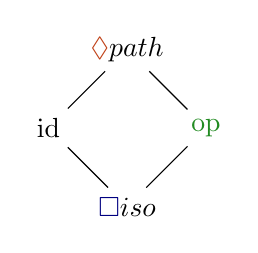
\begin{tikzpicture}[scale=1,baseline=(current bounding box.center)]
      \node (top)  at ( 0, 1) {$\path$};
      \node (bot)  at ( 0,-1) {$\iso$};
      \node (-1)   at (-1, 0) {$\id$};
      \node (1)    at ( 1, 0) {$\op$};
      \draw (top) -- (-1) -- (bot) -- (1) -- (top);
    \end{tikzpicture}

    \begin{array}{r|cccc}
      T \tmeet U
      & \id & \path & \op & \iso\\\hline
      \id & \id & \id & \iso & \iso\\
      \path & \id & \path & \op & \iso\\
      \op & \iso & \op & \op & \iso\\
      \iso & \iso & \iso & \iso & \iso
    \end{array}

    \begin{array}{cr|cccc}
      \multicolumn{2}{c|}{\multirow{2}{*}{$UT$}}
      & \multicolumn{4}{c}{T}\\
      && \id & \op & \iso & \path\\\hline
      \multirow{4}{*}{$U$}
      & \id & \id & \op & \iso & \path\\
      & \op & \op & \id & \iso & \path\\
      & \iso & \iso & \iso & \iso & \path\\
      & \path & \path & \path & \iso & \path
    \end{array}
  \end{mathpar}
  \caption{Tone lattice, meet, and composition}
  \label{fig:tone-ops}
\end{figure*}

\Cref{fig:tone-ops} defines two operators on tones:
\begin{enumerate}
\item Meet $T \tmeet U$ is the greatest lower bound in the lattice ordered $\iso
  < \{\id, \op\} < \path$. This finds the tone of the pairing $\langle f, g\rangle
  : (T \tmeet U)A \to B \times C$ of two functions $f : TA \to B$ and $g : UA
  \to C$.

  %% TODO FIXME: ordering of tone composition is wrong! need to fix this goddamn
  %% everywhere, and I may have already messed up a few places, so double-check
  %% while I'm at it.
\item Composition $UT$ gives the tone of a composed function $g \circ f : UTA
  \to C$ when $f : TA \to B$ and $g : UB \to C$. Equivalently, $(UT)A = U(TA)$
  for any preorder $A$.
\end{enumerate}

We sometimes write $UT$ as $U \tc T$ for clarity. Composition binds tighter than
meet, so $TU \tmeet V = (TU) \tmeet V$.
%
Together, $\tmeet$ and $\tc$ form a semiring whose properties are given in
\cref{fig:tone-op-laws}. \todo{TODO: Reference all those other works which use
  annotations forming a semiring.}

\todo{TODO: check the distribution laws hold!}

\begin{figure*}
  \begin{mathpar}
    \begin{array}{lr@{\hskip 0.5em}c@{\hskip 0.5em}l}
      \multicolumn{4}{c}{\textit{\normalsize Properties of ${}\tmeet{}$}}
      \vspace{2pt}\\
      \text{Associativity} & (T \tmeet U) \tmeet V &=& T \tmeet (U \tmeet V)\\
      \text{Commutativity} & T \tmeet U &=& U \tmeet T\\
      \text{Idempotence} & T \tmeet T &=& T\\
      \path~\text{is identity} & \path \tmeet T &=& T\\
      \iso~\text{absorbs} & \iso \tmeet T &=& \iso\\
    \end{array}

    \begin{array}{lr@{\hskip 0.5em}c@{\hskip 0.5em}l}
      \multicolumn{4}{c}{\textit{\normalsize Properties of ${}\tc{}$}}
      \vspace{2pt}\\
      \text{Associativity} & (TU)V &=& T(UV)\\
      \text{Identity} & \multicolumn{3}{c}{\id \tc T = T = T \tc \id}\\
      \path~ \text{left-absorbs} & T\path &=& \path\\
      \iso~ \text{left-absorbs} & T\iso &=& \iso\\
      \op~ \text{involutive} & \op \tc \op &=& \id\\
    \end{array}

    \begin{array}{lr@{\hskip 0.5em}c@{\hskip 0.5em}l}
      \text{Left distribution} & T (U \tmeet V) &=& TU \tmeet TV\\
      \text{Right distribution} & (T \tmeet U) V &=& TV \tmeet UV
    \end{array}
  \end{mathpar}
  \caption{Properties of tone operators}
  \label{fig:tone-op-laws}
\end{figure*}

\subsection{Monotonicity Types}

\href{https://infoscience.epfl.ch/record/231867/files/monotonicity-types.pdf}{\emph{Monotonicity
    Types}} by Clancy, Miller, and Meiklejohn has similar tables for their
composition $\circ$ and ``contraction'' $+$ operators! However, instead of
bivariance they have constancy, a stricter condition.
%
Constancy corresponds to respecting the \emph{indiscrete ordering} (which sets
$a \le b$ for all $a,b$).\footnote{Indiscreteness and its dual, discreteness,
  are also tones --- that is, functorial transformations on the ordering
  component of a preorder --- but they complicate things, so I omit them.

  Note also that discreteness and $\iso$ coincide on posets; many intuitions
  transfer from one to the other.}
%
Interestingly, because constancy is so much stricter than bivariance, their
composition operator is commutative.

They write $\uparrow$ for $\id$, $\downarrow$ for $\op$, $?$ for $\iso$, and
$\sim$ for constancy. They also add $=$ for the ``tone'' that \emph{only the
  identity function} has. This doesn't fit my framework; it cannot be phrased as
a transformation on orderings. However, it seems related to subtyping.



\section{Tones, categorically}

\newcommand{\elems}[1]{\ensuremath{|{#1}|}}
\newcommand{\elemsfn}[0]{\elems{-}}

%% \renewcommand{\elemsfn}{\mathbold{E}}
%% \renewcommand{\elems}[1]{\elemsfn(#1)}

This section gives a categorical semantics of tones. You may safely skip it.

Let's change perspective. \Cref{sec:tones} defines tones as function
pro\-per\-ties, then gives corresponding pre\-order trans\-form\-ations. Now,
let's define tones as preorder transformations, and derive corresponding
function properties.

\begin{definition}
  $\elemsfn : \Pre \to \Set$ is the functor taking a preorder to its set of
  elements.
\end{definition}

\begin{definition}[Tones]\label{def:tone}
  A tone is a functor $T : \Pre \to \Pre$ such that $\elems{T-} =
  \elemsfn$.\footnote{A more categorical approach might require only a natural
    isomorphism \(\iota : \elems{T-} \isoto \elemsfn\). I'm not yet comfortable
    generalizing that far.} That is, for any preorder $A$ and monotone map $f$,
  \begin{enumerate}
  \item $\elems{TA} = \elems{A}$: tone functors alter a preorder's
    \emph{ordering}, not its elements.
  \item $\elems{Tf} = \elems{f}$: tone functors do not alter functions'
    behavior.
  \end{enumerate}
\end{definition}

%% We say a function $f$ from $A$ to $B$ has tone $T$ iff $f : TA \to B$ is
%% monotone.

%% It's also unclear how to generalize this definition to tones of functors on
%% \Cat{}.

\subsection{Tone composition}

Tone composition $TU$ corresponds to composition of tone functors:

\begin{theorem}
  The composition $TU$ of two tones is itself a tone.
\end{theorem}

\begin{proof} Applying \cref{def:tone}, we have
  \( \elems{T(U-)} = \elems{U-} = \elemsfn \).
\end{proof}


\subsection{The \Tone{} category}

Preorders have a natural partial order, letting $A \le B$ iff $A$ is a
\emph{subpreorder} of $B$ --- that is, if $\fnof{x} x : A \to B$.\footnote{In
  other words, if $A \subseteq B$ and $x \le y : A \implies x \le y : B$.}
%
This lifts pointwise to a partial order on tones: let $T \le U$ iff
$TA \le UA$ for all $A$.
%
As functors, tones also form a category, \Tone{}, with natural transformations
as morphisms. However, \Tone{} is but a fa\c{c}ade over this partial order:

\begin{theorem} \label{thm:tone-poset}
  \[T \le U \iff \exists \eta : \Tone(T, U) \iff \exists! \eta : \Tone(T,U)\]
\end{theorem}

\begin{proof}
  Expanding definitions, $T \le U$ means $\fnof{x} x : TA \to
  UA$ for all $A : \Pre$. By \cref{lem:tone-transformations-are-id},
  any $\eta : \Tone(T,U)$ is of the form $\eta_A = \fnof{x} x : TA
  \to UA$.
\end{proof}

The crux here is that natural transformations between tones are \emph{boring}:
\begin{lemma}\label{lem:tone-transformations-are-id}
  For any natural transformation $\eta : T \to U$, we have $\eta_A = \fnof{x}
  x$.
\end{lemma}

\begin{proof}
  Let $\mb{1}$ be the singleton preorder $\{\star\}$. Fix some $x : A$. Let $f :
  \mb{1} \to A = \fnof{\star}{x}$. Then by naturality of $\eta$, this square
  commutes:
  %
  \[\tikzset{
    no line/.style={draw=none,
      commutative diagrams/every label/.append style={/tikz/auto=false}}}
  \begin{tikzcd}[sep=3.3em]
    \mb{1} \arrow[r,"\textstyle \eta_{\mb{1}}"] \arrow[d,"\textstyle Tf"]
    & \mb{1} \arrow[d,"\textstyle Uf"]
    \\ TA \arrow[r,"\textstyle\eta_A"]
    & UA
  \end{tikzcd}\]

From \cref{def:tone}, $Tf = f = Uf$; and since $\mb{1}$ is
a singleton, $\eta_{\mb{1}} = \idfn$, thus:
  \[\begin{array}{rlcl}
  & \eta_A \circ Tf &=& Uf \circ \eta_{\mb{1}}\\
  \implies & \eta_A \circ f &=& f\\
  \implies & \eta_A(x) &=& x
  \end{array}\]
\end{proof}


\subsection{The \Tone{} lattice}

\begin{conjecture}
  \Tone{} is a distributive lattice.
\end{conjecture}
\begin{proof}
  \todo{TODO}
\end{proof}

\todo{Isn't $\tmeet$ greatest lower bound / product? Don't we have
  $\vee$ / least upper bound / coproducts? Old stuff:}

Tone meet and composition also have semantic versions. $T \tmeet U$ corresponds
to intersection of relations (noting that the intersection of two reflexive,
transitive relations is itself reflexive and transitive), and $TU$ corresponds
to functor composition.
%
\begin{eqnarray*}
  a \le b : (T \tmeet U)A %% \iff a \le b : A^s \cap A^t
  &\iff& a \le b : TA \wedge a \le b : UA\\
  a \le b : (TU)A &\iff& a \le b : T(UA)
\end{eqnarray*}

\begin{conjecture}
  The intersection of two tones is a tone.
\end{conjecture}
\begin{proof}
  \todo{TODO}
\end{proof}

\begin{conjecture}
  The definitions of meet and compose in \cref{fig:tone-ops} coincide with their
  semantic definitions, applied to the semantic interpretation of $\id$, $\op$,
  $\path$, and $\iso$.
\end{conjecture}


\section{An aside on overline notation}

\newcommand{\xbar}[2]{\overline{#2}^{\hspace{.5pt}#1}}
%\renewcommand{\xbar}[2]{\prescript{#1}{}{\vv{#2}}}
%\renewcommand{\xbar}[2]{{\color{red}{\left(#2\right)}_{#1}}}

\newcommand{\Expr}{\Phi}
\newcommand{\Ix}[1]{#1}
\newcommand{\Ex}{{x}}
\newcommand{\Ay}{{A}}

\todo{TODO: Consider instead $\left(\Expr\right)_i$ notation, which I think is
  also a pre-existing convention.}

An overlined and superscripted meta-expression $\xbar{i}{\Expr(i)}$ represents a
sequence (of unspecified length) indexed by $i$. The index $i$ clarifies which
bits are repeated \emph{with variation}, and which \emph{without}. For example:

\begin{center}
  \begin{tabular}{ccl}
    $\xbar{\Ix{i}}{\Ex_{\Ix{i}} : \Ay_{\Ix{i}}}$
    & stands for
    & $\Ex_{\Ix{1}} : \Ay_{\Ix{1}},\, \Ex_{\Ix{2}} : \Ay_{\Ix{2}},\, ...,\, \Ex_{\Ix{n}} : \Ay_{\Ix{n}}$
    \vspace{.5em}\\
    $\xbar{\Ix{i}}{\Ex_{\Ix{i}} : \Ay}$
    & stands for
    & $\Ex_{\Ix{1}} : \Ay,\hspace{0.6em} \Ex_{\Ix{2}} : \Ay,\hspace{0.6em} ...,\, \Ex_{\Ix{n}} : \Ay$
  \end{tabular}
\end{center}

This resembles the usual notation for sums of sequences, but with the bounds
left implicit. For example, $\sum_{i} x_iy_i$ can be written
$\sum\left(\xbar{i}{x_iy_i}\right)$ if we take $\sum$ to be a function from
sequences of numbers to numbers.%
%
\footnote{This convention is also influenced by Guy Steele's talk on Computer
  Science Metanotation. In his talk, Guy analyses ``overline notation'' --- the
  use of $\overline{\Expr(i)}$ to stand for a sequence $\Expr(1), \Expr(2), ...,
  \Expr(n)$. Inspired by quasiquotation in Lisp, he proposes using underlines to
  indicate parts which are repeated \emph{without variation}. Thus $\overline{x
    : A}$ stands for $x_1 : A_1, ..., x_n : A_n$, while $\overline{x :
    \underline{A}}$ stands for $x_1 : A, ..., x_n : A$. In my Lisp experience,
  admittedly more limited than Guy's, quasiquotation is wonderful until you need
  to nest it. Indexes, however, nest nicely.

  There are videos of the talk at
  \href{https://www.youtube.com/watch?v=dCuZkaaou0Q}{Clojure/conj 2017},
  \href{https://www.youtube.com/watch?v=7HKbjYqqPPQ}{PPoPP 2017}, and
  \href{https://www.youtube.com/watch?v=8fCfkGFF7X8&feature=youtu.be&t=37m46s}{Harvard
    University}. There are also
  \href{http://s3.amazonaws.com/erlang-conferences-production/media/files/000/000/755/original/Guy_L._Steele_-_A_Cobbler's_Child.pdf?1510053539}{slides
    from Code Mesh 2017}.}


\section{A tonal sequent calculus}

\newcommand{\T}[1]{#1}

%% "moded" things: hypothesis, types, contexts. mode/tone comes first.
\newcommand{\mtp}[2]{\left[#1\right] #2}
\newcommand{\mcx}[2]{\left[#1\right] #2}
%\renewcommand{\mcx}[2]{#1 #2} % Would need to re-parenthesize some use-sites.
\newcommand{\extend}[2]{{#1},\, {#2}}

\begin{mathpar}
  \mcx{T}{\xbar{i}{\mtp{U_i}{A_i}}} = \xbar{i}{\mtp{TU_i}{A_i}}\\

  \infer[Hypothesis]{T \le \id}{\extend{\GG}{\mtp{T}{A}} \vdash A}

  \infer[$T$-Right]{\GG \vdash A}{\mcx{T}{\GG} \vdash \T{T} A}

  \infer[$T$-Left]
        {\extend{\GG}{\mtp{TU}{A}} \vdash C}
        {\extend{\GG}{\mtp{T}{\T{U}A}} \vdash C}

  \infer[Weakening]{\extend{\GG}{\mtp{T}{A}} \vdash C \\ U \le T}
        {\extend{\GG}{\mtp{U}{A}} \vdash C}

  \infer[Contraction]
        {\extend{\GG}{\mtp{T}{A},\, \mtp{U}{A}} \vdash C}
        {\extend{\GG}{\mtp{T \tmeet U}{A}} \vdash C}

  \infer[Cut]{\GG \vdash A \\ \extend{\Delta}{\mtp{T}{A}} \vdash C}
        {\extend{\mcx{T}{\GG}}{\Delta} \vdash C}
\end{mathpar}

Jason Reed sent me these rules for a sequent calculus, where $\T{T} A$ is the
type internalizing the tone functor $T$ applied to the type $A$. \todo{TODO:
  this notation is convenient but slightly confusing. elucidate it.} I aim to
adapt this into a natural-deduction-style system with proof terms, i.e.\ a
simply typed $\lambda$-calculus.


\section{A bidirectional \texorpdfstring{$\lambda$}{lambda}-calculus with tone inference}

\newcommand{\tpcolor}{}%\color{Green}}
\newcommand{\tmcolor}{}%\color{ACMDarkBlue}}
\newcommand{\cxcolor}{}%\color{ACMPurple}}

\newcommand{\subtype}{\le}
\newcommand{\strips}{\prec}

\newcommand{\uh}[2]{#1 : #2}            % unmoded/toneless hypothesis
\newcommand{\h}[3]{\uh{#1}{\mtp{#2}{#3}}}
\newcommand{\infers}[3]{{\tmcolor#1} \Rightarrow {\cxcolor#2} \vdash {\tpcolor#3}}
\newcommand{\checks}[3]{{\tmcolor#1} \Leftarrow {\cxcolor#2} \vdash {\tpcolor#3}}

\newcommand{\ein}[2]{\textsf{in}_{#1}\:{#2}}
\newcommand{\cto}{\shortrightarrow}
\newcommand{\ecase}[1]{\mb{case}~{#1}~\mb{of}~\,}
\newcommand{\emptycx}{\varepsilon}

\newcommand{\mdist}[2]{#1 \equiv #2}
\newcommand{\mbinop}{\oast}
\newcommand{\adjoint}[2]{#1 \dashv #2}

%% \renewcommand{\infers}[3]{#2 \vdash #1 \Rightarrow #3}
%% \renewcommand{\checks}[3]{#2 \vdash #1 \Leftarrow #3}

%% \renewcommand{\infers}[3]{#1 \Rightarrow {#3} \dashv {#2}}
%% \renewcommand{\checks}[3]{#1 \Leftarrow {#3} \dashv {#2}}
%% \renewcommand{\extend}[2]{{#2},\, {#1}}
%% \renewcommand{\uh}[2]{#2\,#1}

\begin{mathpar}
  \begin{array}{rcclr}
    \text{variables} & x\vspace{1pt}\\
    \text{base types} & P
    \vspace{0.5em}\\

    \text{tones} & T,U,V & \bnfeq & \id \pipe \op \pipe \path \pipe \iso
    \vspace{1pt}\\
    \text{cartesian ops} & \mbinop &\bnfeq& {+} \pipe {\x}
    \vspace{1pt}\\
    \text{types} & A,B,C
    &\bnfeq& P \pipe \isof{A} \pipe \opof{A} \pipe A \to B \pipe A \mbinop B
    \vspace{0.5em}\\

    \text{inferred terms} & e
    &\bnfeq& x \pipe e\;m \pipe \pi_i\;e \pipe m : A \vspace{1pt}\\
    \text{checked terms} & m,n
    &\bnfeq& e \pipe \fnof{x} m \pipe (m,n) \pipe \ein{i}{m}\\
    &&\bnfcont& \mb{let}~x = e~\mb{in}~ m\\
    &&\bnfcont& \ecase{e} \xbar{i}{\ein{i}{x} \cto m_i}
    \vspace{0.5em}\\

    \text{contexts} & \GG
    &\bnfeq& \emptycx \pipe \extend{\GG}{\h{x}{T}{A}}\vspace{1pt}\\
    \text{judgments} & J
    &\bnfeq& \checks{m}{\GG}{A} & \text{type checking}\\
    &&\bnfcont& \infers{e}{\GG}{A} & \text{type inference}\\
    &&\bnfcont& \adjoint{T}{U} \pipe T \le U & \text{tone relations}
    \\
    &&\bnfcont& \mtp{T}{A} \subtype B
    \pipe \mtp{T}{A} \strips B
    & \text{subtyping}
  \end{array}
\end{mathpar}

\todo{TODO: explain my various abuses of notation, e.g. $\mcx{T}{\GG}$ and
  $\GG_1 \tmeet \GG_2$}


\subsection{Typing rules}

\subsubsection{Inferred forms}
%
\begin{mathpar}
  %% ---- inferring forms ----
  %% checking -> inferring by annotation
  \infer{\checks{m}{\GG}{A}}{\infers{m : A}{\GG}{A}}

  %% variables
  \infer{ }{\infers{x}{\h{x}{\id}{A}}{A}}

  %% projection
  \infer{\infers{e}{\GG}{A} \\ \mtp{T}{A} \strips B_1 \x B_2}
        {\infers{\pi_i\;e}{\mcx{T}{\GG}}{B_i}}

  %% application
  \infer{\infers{e}{\GG_1}{A}
         \\ \mtp{T}{A} \strips B \to C
         \\ \checks{m}{\GG_2}{B}}
        {\infers{e\; m}{\mcx{T}{\GG_1} \tmeet \GG_2}{C}}
\end{mathpar}

\subsubsection{Checking forms}
%
\begin{mathpar}
  %% ---- checking forms ----
  %% inferring -> checking by subtyping
  \infer{\infers{e}{\GG}{A} \\ \mtp{T}{A} \subtype B}
        {\checks{e}{\mcx{T}{\GG}}{B}}

  %% mode introduction
  \infer{\checks{m}{\GG}{A} \\ T \in \{\iso,\op\}}
        {\checks{m}{\mcx{T}{\GG}}{\T{T} A}}

  %% let-binding
  \infer{\infers{e}{\GG_1}{A} \\ \checks{m}{\extend{\GG_2}{\h{x}{T}{A}}}{C}}
        {\checks{\mb{let}~x = e~\mb{in}~m}{\mcx{T}{\GG_1} \tmeet \GG_2}{C}}

  %% lambdas
  \infer{\checks{m}{\extend{\GG}{\h{x}{T}{A}}}{B} \\ \id \le T}
        {\checks{\fnof{x} m}{\GG}{A \to B}}

  %% pairs
  \infer{\checks{m}{\GG_1}{A_1} \\ \checks{n}{\GG_2}{A_2}}
        {\checks{(m,n)}{\GG_1 \tmeet \GG_2}{A_1 \x A_2}}

  %% injection
  \infer{\checks{m}{\GG}{A_i}}
        {\checks{\ein{i}{m}}{\GG}{A_1 + A_2}}

  %% case analysis
  \infer{\infers{e}{\GG}{A} \\
         \mtp{T}{A} \strips B_1 + B_2 \\
         \fapremise{i}
         \checks{m_i}{\extend{\GG_i}{\h{x}{U_i}{B_i}}}{C}}
        {\checks{\ecase{e} \xbar{i}{\ein{i}{x} \cto m_i}}
          {\textstyle\bigmeet_i\left( \mcx{U_iT}{\GG} \tmeet \GG_i \right)}
          {C}}
\end{mathpar}


\subsection{Tone judgments}

\todo{TODO: Explain judgment $s \le t$, for tone ordering, and $\adjoint{s}{t}$,
  for tone adjunction.}
%
\begin{mathpar}
\adjoint{\id}{\id}

\adjoint{\op}{\op}

\adjoint{\path}{\iso}

\infer{}{T \le T}

\infer{}{\iso \le T}

\infer{}{T \le \path}
\end{mathpar}



\subsection{Subtyping}

\todo{TODO: Explain why we use tone-annotated subtyping.}

\todo{TODO: Explain the intended algorithmic reading here. Note that we
  case-analyse both $A$ and $B$, and argue that the order we apply the rules in
  shouldn't matter. Eventually I'll want to prove soundness (wrt semantics) \&
  completeness (wrt some more declarative system).}

\newcommand{\focus}[1]{{\color{Rhodamine}#1}}

In $\mtp{T}{A} \subtype {B}$, the types $A$ and $B$ are inputs, and the tone $T$
is output. In each rule I've marked the connective being analysed in
\focus{pink}.
%
\begin{mathpar}
  \infer[refl]{}{\mtp{\id}{A} \subtype {A}}

  \infer[t-right]
        {\mtp{T}{A} \subtype B}
        {\mtp{UT}{A} \subtype \T{\focus{U}} B}

  \infer[t-left]
        {\mtp{T}{A} \subtype B \\ \adjoint{U}{V}}
        {\mtp{TU}{\T{\focus{V}} A} \subtype B}

  %% Products and sums
  \infer[cartesian distribution]
        {\mtp{T}{A_1} \subtype A_2 \\ \mtp{U}{B_1} \subtype B_2}
        {\mtp{T \tmeet U}{A_1 \mathop{\focus\mbinop} B_1}
          \subtype A_2 \mathop{\focus\mbinop} B_2}
\end{mathpar}

The semantic justification for \textsc{adjoint} is as follows.
%
Note that $\fnof{x} x : VA \to VA$. Applying $U \dashv V$ we have $\fnof{x} x :
UVA \to A$, thus $UVA \le A$, and so finally $TUVA \le TA \le B$. \todo{Clean up
  this explanation. Explain that we use adjunction rather than $st \le \id$
  directly because adjunction gives us the \emph{most informative} result; $st
  \le \id$ is declarative, $\adjoint{t}{s}$ is algorithmic. Give explanations
  for each other rule as well.}

Function subtyping, $\mtp{T}{A_1 \mathrel{\focus{\to}} B_1} \subtype A_2
\mathrel{\focus{\to}} B_2$, has four rules, one for each tone $T$ produced by
$\mtp{T}{B_1} \subtype B_2$:
%
\begin{mathpar}
  \infer{\id \le T \\ \mtp{T}{A_2} \subtype A_1 \\ \mtp{\id}{B_1} \subtype B_2}
        {\mtp{\id}{A_1 \to B_1} \subtype A_2 \to B_2}

  \infer{\op \le T \\ \mtp{T}{A_2} \subtype A_1 \\ \mtp{\op}{B_1} \subtype B_2}
        {\mtp{\op}{A_1 \to B_1} \subtype A_2 \to B_2}

  \infer{\path T = \path \\ \mtp{T}{A_2} \subtype A_1 \\ \mtp{\path}{B_1} \subtype B_2}
        {\mtp{\path}{A_1 \to B_1} \subtype A_2 \to B_2}

  \infer{\mtp{\path}{A_2} \subtype A_1 \\ \mtp{\iso}{B_1} \subtype B_2}
        {\mtp{\iso}{A_1 \to B_1} \subtype A_2 \to B_2}
\end{mathpar}

The premise $\path T = \path$ of the third rule holds for $T \ne \iso$ in our system;
however, $\path T = \path$ captures more exactly \emph{why} the rule is valid.
\todo{TODO: Give proofs each of these rules are valid.}

\todo{Are there also more precise/suggestive versions of the other premises? Can
  the $U \le T$ constraints be turned into ``composing with $V$ is $\ge \id$'',
  for some choice of $V$ depending on $U$?}

Subtyping at base types will depend on the base types you choose. Frequently,
some base types' preorders will be symmetric (or even discrete, $x \le y \iff x
= y$), and therefore equivalence relations. Let ``$P~\text{equiv}$'' hold if
$P$'s order is symmetric. Then the following refinement of \textsc{refl} is
useful:
\[ \infer{P~\text{equiv}}{\mtp{\path}{P} \subtype P} \]


\subsection{Mode stripping}

$\mtp{T}{A} \strips B$ is a specialization of $\mtp{T}{A} \subtype B$ which
strips off modal operators on $A$, turning them into transformations on $T$. As
in subtyping, $A$ is an input and $T$ an output; however, $B$ is now an output.
%
\begin{mathpar}
  \infer{\fapremise{T,B} A \ne \T{T} B}{\mtp{\id}{A} \strips A}

  \infer{\mtp{T}{A} \strips B \\ \adjoint{U}{V}}
        {\mtp{TU}{\T{V} A} \strips B}
\end{mathpar}

\todo{TODO: note that we cannot strip the mode $\path$. $\path$ is basically a
  pariah; we cannot eliminate it through mode stripping, and we don't have an
  explicit elimination rule.}


\subsection{Tones and the \texorpdfstring{$\fn$}{lambda} rule}

%% TODO: check tone composition order here!
Here are two more general variations on the $\fn$ rule I've considered:
%
\begin{mathpar}
  \infer[Fn-1]
        {\checks{m}{\extend{\GG}{\h{x}{T}{A}}}{B} \\ A \le \mtp{T}{A}}
        {\checks{\fnof{x}{m}}{\GG}{A \to B}}

  \infer[Fn-2]
        {\checks{m}{\extend{\GG}{\h{x}{U}{A}}}{B}
         \\ \mtp{T}{A} \subtype A
         \\ \id \le T U}
        {\checks{\fnof{x} m}{\GG}{A \to B}}
\end{mathpar}
\textsc{Fn-1} requires a new judgment, $A \le \mtp{T}{B}$, where $A,B,T$ are all
inputs; this doesn't seem difficult to define, but it's Yet Another Subtyping
Judgment. \textsc{Fn-2} avoids this, but is much less easy to explain.

However, it's not clear to me I need to generalize the $\fn$ rule. The reason I
thought I did was to justify something like the following:
\begin{mathpar}
  \infer*{\infer*{\vdots}
           {{\extend{\GG}{\h{x}{\iso}{A}}} \vdash {m} : {B}}}
         {{\GG} \vdash {\fnof{x}{m}} : {\T{\iso} A \to B}}
\end{mathpar}

But this \emph{could} check as follows:
\begin{mathpar}
  \infer*{\infer*{\vdots}{\checks{m}{\extend{\GG}{\h{x}{T}{(\T{\iso} A)}}}{B}}
          \\ \id \le T}
         {\checks{\fnof{x}{m}}{\GG}{\T{\iso} A \to B}}
\end{mathpar}

So the crucial question is: can we always substitute $\h{x}{\id}{\T{\iso} A}$
for $\h{x}{\iso}{A}$?
%
It would suffice to prove the subtyping and substitution principles given in
\cref{sec:principles}. Can we prove these with our original, subtyping-less
$\lambda$ rule?


\section{Pattern matching}

\newcommand{\pwild}{\_}
\newcommand{\pcheck}[3]{#1 : #2 \vdash #3}
%\newcommand{\armcheck}[6]{#1 \cto #2 : #3 \vdash {#4}^{#5} >\!\!> #6}
\newcommand{\armcheck}[6]{#1 \cto #2 \Leftarrow \mtp{#3}{#4};\, #5 \vdash #6}
\newcommand{\mprecx}[2]{#1 #2}

\[\begin{array}{rccl}
  \text{patterns} & p,q
  &\bnfeq& x ~|~ (p,q) ~|~ \ein{i}{p}
  \vspace{0.5em}\\
  \text{checking terms} & m,n
  &\bnfeq& \ecase{e} \xbar{i}{p_i \cto m_i}
  \vspace{0.5em}\\
  \text{toneless contexts} & \phi,\psi
  &\bnfeq& \emptycx ~|~ \extend{\phi}{\uh{x}{A}}
  \vspace{0.5em}\\
  \text{judgments} & J
  &\bnfeq& \mdist{A}{B \mbinop C}\\
  &&\bnfcont& \pcheck{p}{A}{\phi}\\
  &&\bnfcont& \armcheck{p}{m}{T}{A}{\GG}{C}
\end{array}\]

\vspace{.5em} The types in toneless contexts $\phi$ aren't annotated with tones.
\todo{TODO: Explain why and when we use toneless contexts. Explain
  $\mprecx{\vv{T}}{\phi}$ notation for a context split into its tones and its
  types.}


\subsection{Distributing modes}

The pattern $(x,y)$ matches values of type $A \x B$. But how shall we match
values of type $\T{T}(A \x B)$?
%
%We might add a pattern, $\mb{wrap}_T\:p$, matching values of type $\T{T} A$.
%Then $\mb{wrap}_T\:(x,y)$ would match values of type $\T{T}(A \x B)$.
%But do we \emph{need} a $\mb{wrap}_T$ annotation?
Well, \Cref{thm:tones-monoidal} says $\T{T} (A \x B) \isoto \T{T} A \x \T{T} B$.
So $(x,y)$ can \emph{also} match $\T{T}(A \x B)$, yielding $x : \T{T} A$ and $y
: \T{T} B$.
%
To type-check this, we'll need a judgment $\mdist{A}{B \mbinop C}$ for
distributing modes over a cartesian operator $\mbinop$ (either $\x$ or $+$).
Here $A$ is an input and $B$, $C$ are outputs.
%
\begin{mathpar}
  \infer{ }{\mdist{A \mbinop B}{A \mbinop B}}

  \infer{\mdist{A}{B \mbinop C}}{\mdist{\T{T} A}{\T{T} B \mbinop \T{T} C}}
\end{mathpar}


\subsection{Typing patterns}

The judgment $\pcheck{p}{A}{\phi}$ corresponds to a \Pre-morphism $A \to 1 +
\phi$. It means that the pattern $p$, when it matches a value of type $A$,
produces values for $\phi$'s variables.
%
\begin{mathpar}
  \infer{ }{\pcheck{x}{A}{\uh{x}{A}}}

  \infer{\mdist{A}{A_1 + A_2} \\ \pcheck{p}{A_i}{\phi}}
        {\pcheck{\ein{i}{p}}{A}{\phi}}

  \infer{\mdist{A}{A_1 \x A_2} \\
         \fapremise{i} \pcheck{p_i}{A_i}{\phi_i}\\
         \phi_1,\phi_2~\text{disjoint}}
        {\pcheck{(p_1, p_2)}{A}{\phi_1,\phi_2}}
\end{mathpar}

%% To handle non-linear patterns, or patterns with gu\-ard expressions, the
%% morphism would also need an input context $\GG$. I consider this in
%% \cref{sec:patterns-with-guards}.


\subsection{Typing \mb{case}-analysis}

Typing \mb{case} as a single rule is complicated:
%
\[
\infer{
  \infers{e}{\GG}{A} \\
  \fapremise{i} \pcheck{p_i}{A}{\phi_i} \\
  \fapremise{i}
  \checks{m_i}{\GG_i, \mprecx{\vvsub{T}{i}}{\phi_i}}{C}
}{
  \checks
      {\ecase{e} \xbar{i}{p_i \cto m_i}}
      {\bigmeet_i\left(\GG_i \tmeet \mcx{\bigmeet\!\vvsub{T}{i}}{\GG}\right)}
      {A}}
\]

We can split this up using a helper judgment, $\armcheck{p}{m}{T}{A}{\GG}{C}$,
corresponding to a morphism $TA \x \GG \to 1 + C$. This says that the arm $p
\cto m$ matches a scrutinee of type $A$ that it uses at tone $T$, along with
variables in $\GG$, to produce (if it matches) a result of type $C$. Then we
have:
%
\begin{mathpar}
  \infer{\pcheck{p}{A}{\phi} \\
         \checks{m}{\GG, \mprecx{\vv{T}}{\phi}}{C}
  }     {\armcheck{p}{m}{\textstyle\bigmeet\!\vv{T}}{A}{\GG}{C}}

  \infer{\infers{e}{\GG}{A} \\
         \fapremise{i} {\armcheck{p_i}{m_i}{T_i}{A}{\GG_i}{C}}
  }{\checks
    {\ecase{e} \xbar{i}{p_i \cto m_i}}
    {\bigmeet_i \left( \mcx{T_i}{\GG} \tmeet \GG_i \right)}
    {C}}
\end{mathpar}


\subsection{Why do we need both stripping and distribution?}

Can we also use modal distribution instead of modal stripping in our typing
rules for expressions? Not quite. We can rewrite the tuple-projection rule:
\begin{mathpar}
  \infer{\infers{e}{\GG}{A} \\ \mdist{A}{A_1 \x A_2}}
        {\infers{\pi_i\;e}{\GG}{A_i}}
\end{mathpar}

However, we cannot rewrite function application (shown below) this way; in
general, $\T{T}(A \to B) \not\equiv \T{T} A \to \T{T} B$. (In particular for $T
\in \{\iso,\path\}$.) So it seems there is no choice but to use subtyping.

\begin{mathpar}
  \infer{\infers{e}{\GG_1}{A}
         \\ {\color{ACMRed} \mtp{T}{A} \strips B \to C}
         \\ \checks{m}{\GG_2}{B}}
        {\infers{e\; m}{\mcx{T}{\GG_1} \tmeet \GG_2}{C}}
\end{mathpar}

\todo{TODO: explain why using modal stripping for pattern matching doesn't work,
  with the $(x,(y,z))$ versus $A \x \Box(B \x C)$ example.}

\todo{TODO: explain why using modal stripping rather than distribution for the
  tuple projection rule is fine, because of the adjunction between \path{} and
  \iso{}.}


\subsection{Case analysis with guarded arms}

%% TODO: rewrite these judgments.

\newcommand{\armif}[3]{#1 ~\mb{if}~ #2 \cto #3}
\newcommand{\armifcheck}[7]{%
  \armif{#1}{#2}{#3} \Leftarrow \mtp{#4}{#5};\, {#6} \vdash #7}

%% \renewcommand{\armifcheck}[7]{%
%%   \armif{#1}{#2}{#3} \Leftarrow #5^{#6} \rightsquigarrow #7 \dashv {\,#4}}

\[\begin{array}{rccl}
  \text{checking expressions} & m
  &\bnfeq& \ecase{e} \xbar{i}{\armif{p_i}{m_i}{n_i}}
  \vspace{.5em}\\
  \text{judgments}& J &\bnfeq& \armifcheck{p}{m}{n}{T}{A}{\GG}{C}
\end{array}\]

\begin{mathpar}
  \infer{
    \pcheck{p}{A}{\phi} \\
    \checks{m}{\GG_1, \mprecx{\vv{T}}{\phi}}{\isof{2}} \\
    \checks{n}{\GG_2, \mprecx{\vv{U}}{\phi}}{C}
  }{\textstyle
    \armifcheck{p}{m}{n}
               {\bigmeet\!\vv{T} \tmeet \bigmeet\!\vv{U}}
               {A}{\GG}{C}}

  \infer{
    \infers{e}{\GG}{A} \\
    \fapremise{i} \armifcheck{p_i}{m_i}{n_i}{T_i}{A}{\GG_i}{C}
  }{\checks
    {\ecase{e} \xbar{i}{\armif{p_i}{m_i}{n_i}}}
    {\textstyle\bigmeet_i\left( \mcx{T_i}{\GG} \tmeet \GG_i \right)}
    {C}}
\end{mathpar}


\subsection{Patterns with embedded guards}
\label{sec:patterns-with-guards}

\newcommand{\pif}[2]{{#1}~\mb{if}~{#2}}
\newcommand{\pcheckio}[5]{#1 : \mtp{#2}{#3} \vdash #4 \vdash #5}

\[\begin{array}{rccl}
  \text{patterns} & p,q
  &\bnfeq& \pif{p}{m}
  \vspace{0.5em}\\
  \text{judgments} & J &\bnfeq& \pcheckio{p}{T}{A}{\GG}{\phi}
\end{array}\]

\vspace{\parsep}

Now that patterns can contain expressions, our pattern typing judgment takes an
input context $\GG$, becoming $\pcheckio{p}{T}{A}{\GG}{\phi}$. This corresponds
to a morphism $\GG \x TA \to 1 + \phi$. \todo{However, at this point our rules
  get so complicated I don't trust them without a proof:}

\begin{mathpar}
  \infer{x \not\in \phi}{
    \pcheckio{x}{\id}{A}{\mprecx{\vv{\path}}{\phi}}{x : A}}

  \infer{\mdist{A}{A_1 + A_2} \\
         \pcheckio{p}{T}{A_i}{\GG}{\phi}}
        {\pcheckio{\ein{i}{p}}{T}{A}{\GG}{\phi}}

  \infer{\mdist{A}{B \x C} \\
         \pcheckio{p}{T}{B}{\GG_1}{\phi} \\
         \pcheckio{q}{U}{C}{\GG_2, \mprecx{\vv{V}}{\phi}}{\psi}
  }{\textstyle
    \pcheckio{(p,q)}
             {\left(\id \tmeet \bigmeet\!\vv{V}\right) T \tmeet U}
             {A}
             {\mcx{\id \tmeet \bigmeet\!\vv{V}}{\GG_1} \tmeet \GG_2}
             {\phi, \psi}}

  \infer{\pcheckio{p}{T}{A}{\GG_1}{\phi} \\
         \checks{m}{\GG_2, \mprecx{\vv{U}}{\phi}}{\isof{2}}
  }{\textstyle
    \pcheckio
        {\pif{p}{m}}
        %{\left(\id \tmeet \path{\bigmeet\!\vv{U}} \right) T}
        {T \tmeet \path\bigmeet\!\vv{U}T}
        {A}
        {\mcx{\id \tmeet \path\bigmeet\!\vv{U}}{\GG_1} \tmeet \mcx{\path}\GG_2}
        {\phi}}
\end{mathpar}

Now we update the rules for $\armcheck{p}{m}{T}{A}{\GG}{C}$ to pass through $\GG$ to the pattern:
%
\begin{mathpar}
  \infer{\pcheckio{p}{T}{A}{\GG_1}{\phi} \\
         \checks{m}{\GG_2, \mprecx{\vv{U}}{\phi}}{C}}
        {\armcheck{p}{m}{T}{A}{\mcx{\bigmeet\!\vv{U}}{\GG_1} \tmeet \GG_2}{C}}
\end{mathpar}

%% \subsection{Old work}

%% \newcommand{\pinfer}[5]{#1 : #2 \vdash #3^{#4} \dashv #5}

%% Judgment: $\pinfer{p}{\GG}{A}{s}{\Delta}$. \todo{TODO: what's an input, what's
%%   an output? I think $s$ and the tones on $\GG$ are outputs? so the only inputs
%%   are $A$ and the types in $\GG$.}

%% \begin{mathpar}
%%   %% this is wrong
%%   \infer{x \not\in \GG}
%%         {\pinfer{x}{\GG}{A}{s}{x : A^s}}

%%   \infer{\h{x}{t}{A} \in \GG
%%          \\ \text{\todo{TODO}}
%%          \\ A~\text{decidable} }
%%         {\pinfer{x}{\GG}{A}{s}{\emptycx}}

%%   \infer{A^{t} \strips B_1 \x B_2
%%          \\ \pinfer{p}{\GG}{B_1}{?}{\Delta_1}
%%          \\ \pinfer{q}{\GG,\Delta_1}{B_2}{?}{\Delta_2} }
%%         {\pinfer{(p,q)}{\GG}{A}{s}{\Delta_1, \Delta_2}}
%% \end{mathpar}


\section{Declarative rules}

\todo{This is where I'm stashing important inference rules, stated in a way that
  makes them obviously valid, but leaves non-obvious how to algorithmically
  check them.}

\subsection{Subtyping and type equivalence}

%% TODO: rewrite these judgments
%% TODO: use \T!

Type equivalence $A \equiv B$ is a synonym for $A \le B \tmeet B \le A$. Let $A
\le B$ be the preorder generated by:
%
\begin{mathpar}
  \infer{T \le U}{TA \le UA}

  \infer{A \le B}{TA \le TB}

  \infer{}{T(UA) \equiv (TU)A}

  \infer{}{T(A \mbinop B) \equiv TA \mbinop TB}

  \infer{}{\opof{(A \to B)} \equiv \opof{A} \to \opof{B}}

  \infer{}{A \to \isof{B} \equiv \isof{(A \to \isof{B})}}

  \infer{}{\isof{(A \to B)} \le \isof{A} \to \isof{B}}

  \infer{A_1 \le B_1 \\ A_2 \le B_2}{A_1 \mbinop A_2 \le B_1 \mbinop B_2}

  \infer{A_2 \le A_1 \\ B_1 \le B_2}{A_1 \to B_1 \le A_2 \to B_2}
\end{mathpar}

\begin{conjecture}
  This judgment is complete for subpreordering relationships of the form $TA \le
  B$ where $\path$ does not occur in $A$ or $B$ (but may occur in $T$).
\end{conjecture}

\todo{TODO: check we can derive the algorithmic function subtyping rules.
  $\isof{(A \to B)} \le \isof{A} \to \isof{B}$ handles one of the cases;
  $\opof{(A \to B)} \equiv \opof{A} \to \opof{B}$ handles another; what about
  the last one?}

\todo{As I originally conceived of this system, there was no type $\pathof{A}$
  internalizing the $\path$ tone, so I imagine it's not complete for types of
  that form. In fact, there are \emph{no} rules above about $\path$
  specifically.}

\todo{Here are some more valid rules, but do I need them?}
%
\begin{mathpar}
  \infer{}{\idof{A} \equiv A}

  \infer{T,U \in \{\iso, \path\}}
        {A \to UB \equiv T(A \to UB)}

  \infer{T \in \{\iso, \path\} \\ \adjoint{U}{V}}
        {T(UA \to B) \equiv T(A \to VB)}
\end{mathpar}


\section{Metatheory}
\subsection{Weakening, subtyping, and substitution}
\label{sec:principles}

We wish to prove admissible the following rules:
%
\begin{mathpar}
  \infer[tone weakening]
        {\checks{m}{\GG}{A}}
        {\checks{m}{\GG \tmeet \GG'}{A}}

  \infer[subtyping left]
        {\checks{m}{\GG, \h{x}{T}{A}}{C} \\ TA \le UB}
        {\checks{m}{\GG, \h{x}{U}{B}}{C}}

  \infer[subtyping right]
        {\checks{m}{\GG}{A} \\ TA \le B}
        {\checks{m}{\mcx{T}{\GG}}{B}}

  \infer[substitution]
        {\infers{e}{\GG_1}{A}
         \\ TA \le UB
         \\ \checks{m}{\GG_2, \h{x}{U}{B}}{C}}
        {\checks{m[e/x]}{\mcx{T}{\GG_1} \tmeet \GG_2}{C}}
\end{mathpar}

\todo{TODO: Doesn't \textsc{tone weakening} follow from \textsc{subtyping
    left}?}


%% \section{Typing rules for tone synthesis}

%% \newcommand{\hilited}{\color{blue}}
%% \renewcommand{\hilited}{\color{Rhodamine}}
%% \renewcommand{\hilited}{\color{Emerald}}

%% The declarative typing rule for \textbf{let}, which internalizes the
%% substitution principle, is:
%% \begin{mathpar}
%%   \infer{
%%     \GG \vdash \h{M}{B}{s}
%%     \quad
%%     \GG, \h{x}{B}{s} \vdash \h{N}{C}{t}
%%   }{
%%     \GG \vdash \textbf{let}~ x = M ~\textbf{in}~ \h{N}{C}{t}
%%   }
%% \end{mathpar}

%% This can be bidirectionalized as follows, recalling that in a context, the
%% variables' types are inputs, but their tones are outputs:
%% \begin{mathpar}
%%   \infer{
%%     \xbar{i}{\h{x_i}{A_i}{\hilited s_i}} \vdash M \Rightarrow B
%%     \quad
%%     \xbar{i}{\h{x_i}{A_i}{\hilited t_i}},\, \h{y}{B}{\hilited u}
%%     \vdash N : C
%%   }{
%%     \xbar{i}{\h{x_i}{A_i}{\hilited (s_i \tc u) \tmeet t_i}}
%%     \vdash \textbf{let}~ y = M ~\textbf{in}~ N : C
%%   }
%% \end{mathpar}

%% Some more bidirectionalized inference rules:

%% \begin{mathpar}
%%   \infer{
%%     \xbar{i}{\h{x_i}{A_i}{s_i}} \vdash M : A
%%     \quad
%%     \xbar{i}{\h{x_i}{A_i}{t_i}} \vdash N : B
%%   }{\xbar{i}{\h{x_i}{A_i}{s_i \tmeet t_i}} \vdash (M,N) : A \x B}

%%   \infer{\xbar{i}{\h{x_i}{A_i}{s_i}} \vdash M : B_1 \x B_2}
%%         {\xbar{i}{\h{x_i}{A_i}{s_i}} \vdash \pi_i\;M : B_i}
%%   \\

%%   \infer{\xbar{i}{\h{x_i}{A_i}{s_i}}, \h{y}{B}{t} \vdash M : C}
%%         {\xbar{i}{\h{x_i}{A_i}{s_i}} \vdash \fnof{x} M : B \overset{t}{\to} C}

%%   \infer{\xbar{i}{\h{x_i}{A_i}{s_i}} \vdash M : B \overset{u}{\to} C
%%          \quad
%%          \xbar{i}{\h{x_i}{A_i}{t_i}} \vdash N : B}
%%         {\xbar{i}{\h{x_i}{A_i}{s_i \tmeet (t_i \tc u)}} \vdash M\;N : C}
%%   \\

%%   \infer{\xbar{i}{\h{x_i}{A_i}{s_i}} \vdash M : C}
%%         {\xbar{i}{\h{x_i}{A_i}{s_i \tc \iso}} \vdash \textbf{box}\;M : \square C}

%%   \infer{\xbar{i}{\h{x_i}{A_i}{s_i}} \vdash M : \square B
%%          \quad
%%          \xbar{i}{\h{x_i}{A_i}{t_i}, \h{y}{B}{u}} \vdash N : C
%%          \quad \iso \le u}
%%         {\xbar{i}{\h{x_i}{A_i}{(s_i \tc \path) \tmeet t_i}} \vdash
%%           \textbf{let box}~ x = M ~\textbf{in}~ N : C}
%% \end{mathpar}

%% \todo{TODO: Even more inference rules. Case analysis, in particular.}

%% \todo{TODO?: Some way of giving tone annotations that doesn't need so many
%%   overlines?}


%% \section{Category and preorder theory}

%% \[
%% \begin{array}{clll}
%%   \multicolumn{1}{l}{\textbf{Notation}}
%%   & \multicolumn{1}{l}{\textbf{Name}}
%%   & \multicolumn{1}{l}{\textbf{How to make it}}
%%   & \multicolumn{1}{l}{\textbf{In $\Pre$}}
%%   \\\hline
%%   C^\path
%%   & \text{``localization of $C$''}
%%   & \text{freely add inverses for every morphism}
%%   & \text{equivalence closure}
%%   \\
%%   C^\iso
%%   & \text{``core of $C$''}
%%   & \text{keep only the isomorphisms}
%%   & \text{induced equivalence}
%% \end{array}
%% \]

%% $C^\path$ and $C^\iso$ are groupoids --- categories where every morphism is an
%% isomorphism. I assert but do not prove that $-^\path$ and $-^\iso$ are
%% functorial, $\cat{Cat} \to \cat{Groupoid}$. If we restrict the domain to
%% $\Pre$, the codomain restricts to $\cat{Setoid}$.

%% Diagramatically, leaving inclusion functors unlabeled:
%% {\large\[
%%   \tikzset{
%%     no line/.style={draw=none,
%%       commutative diagrams/every label/.append style={/tikz/auto=false}}}
%%   \begin{tikzcd}[row sep=5em,column sep=4em]
%%     \cat{Cat}
%%     \arrow[d,bend right=40,"\textstyle\path"'{name=A}]
%%     \arrow[d,bend left=40,"\textstyle\iso"{name=C}]
%%     & \Pre
%%     \arrow[d,bend right=40,"\textstyle\path"'{name=A2}]
%%     \arrow[d,bend left=40,"\textstyle\iso"{name=C2}]
%%     \arrow[l]
%%     \\
%%     \cat{Groupoid} \arrow[u,""{name=B}]
%%     & \cat{Setoid} \arrow{u}[name=B2]{} \arrow[l]
%%     %% the \dashv's between adjoint arrows
%%     \arrow[to path={(A) -- (B)\tikztonodes}, no line, near end]{}{\displaystyle\dashv}
%%     \arrow[to path={(B) -- (C)\tikztonodes}, no line]{}{\displaystyle\dashv}
%%     \arrow[to path={(A2) -- (B2)\tikztonodes}, no line, near end]{}{\displaystyle\dashv}
%%     \arrow[to path={(B2) -- (C2)\tikztonodes}, no line]{}{\displaystyle\dashv}
%%   \end{tikzcd}
%% \]}

%% $-^\path \dashv \mc{U} \dashv -^\iso$ form an \emph{adjoint triple}, where
%% $\mc{U}$ is the inclusion $\cat{Groupoid} \to \cat{Cat}$. \todo{TODO:
%%   Prove this, and explain what adjoint triples are.}
%% %
%% Let $\lozenge = \mc{U}(-^\path)$ and $\square = \mc{U}(-^\iso)$. This adjoint
%% triple implies that $\lozenge$ is a monad, $\square$ a comonad, and that
%% $\lozenge \dashv \square$.

%% Some useful notation:
%% \[\begin{array}{lcl@{\hskip 2em}l}
%%   f : x \to y : A &\iff& f \in A(x,y)
%%   & \text{``$f$ is an $A$-morphism from $x$ to $y$''}\\
%%   f : x \simeq y : A &\iff& f \in A^\iso(x,y)
%%   & \text{``$f$ is an $A$-isomorphism from $x$ to $y$''}\\
%%   f : x \pathto y : A &\iff& f \in A^\path(x,y)
%%   & \text{``$f$ is an $A$-path from $x$ to $y$''}
%% \end{array}\]

%% In $\Pre$ and $\cat{Setoid}$, we can ignore the names of morphisms:
%% \[\begin{array}{lclcl}
%%   x \le y : A &\iff& \exists f \in A(x,y)\\
%%   x \isoto y : A &\iff& x \le y : A^\iso &\iff& x \le y \wedge y \le x : A\\
%%   x \pathto y : A &\iff& x \le y : A^\path
%%   &\iff& \exists\bind{\vec{a}} a_0 = x \wedge a_n = y
%%   \wedge \forall\bind{i} (a_i \le a_{i+1} \vee a_{i+1} \le a_i : A)
%% \end{array}\]

%% I may omit annotations ``$: A$'' when the intended category (groupoid, preorder,
%% setoid) is clear. I \emph{never} omit it in cases such as $x \le y : A^\iso$ or
%% $x \le y : A^\path$ --- that is, where the intended category is the result of
%% applying a functor.

%% \begin{lemma}\label{lem:loccore-1}
%%   Every monotone map $A^\path \to B$ is a monotone map $A \to B^\iso$ and
%%   vice-versa, i.e.
%%   \[ \Pre(A^\path, B) = \Pre(A, B^\iso) \]
%% \end{lemma}

%% \begin{proof} We prove each direction:
%%   \begin{enumerate}
%%   \item Fix $F : A^\path \to B$ and suppose $x \le y : A$; we wish to show $F(x)
%%     \equiv F(y)$. By the definition of $A^\path$, from $x \le y$ we know $x
%%     \equiv y : A^\path$. Then by monotonicity of $F$ we have $F(x) \equiv F(y) :
%%     B$.

%%   \item Fix $F : A \to B^\iso$ and suppose $x \pathto y : A$; we wish to show
%%     $F(x) \le F(y)$. Since $x \pathto y$ there is a sequence $\vec{a}$ such that
%%     $a_0 = x$, $a_n = y$, and $a_i \le a_{i+1} \vee a_{i+1} \le a_i$ for $i$
%%     from 1 to $n-1$. From either case of this last disjunction and the
%%     monotonicity of $F$ we have $F(a_i) \equiv F(a_{i+1})$; by transitivity
%%     $F(x) \equiv F(y)$ and so $F(x) \le F(y)$.
%%   \end{enumerate}
%% \end{proof}

\end{document}
